\uppercase{\section{Experiments}}

\begin{figure*}[t]
\scriptsize
\centering
\setlength{\tabcolsep}{1.5pt}
\begin{tabular}{cccccccccc}
    {}&\mr{2}{\Th{Input}}&\mc{2}{\Th{Grad-CAM}}&\mc{2}{\Th{Grad-CAM++}}&\mc{2}{\Th{Score-CAM}}&\mc{2}{\Th{Ablation-CAM}}\\
    {}&{}&\Th{Baseline}&\Th{Denoised}&\Th{Baseline}&\Th{Denoised}&\Th{Baseline}&\Th{Denoised}&\Th{Baseline}&\Th{Denoised}\\
  %  {\rotatebox{90}{\small Man}}&\includegraphics[width=0.09\textwidth]{fig/fig_cam/original/4862.JPEG}&\includegraphics[width=0.09\textwidth]{fig/fig_cam/baseline/gradcam/4862.JPEG}&\includegraphics[width=0.09\textwidth]{fig/fig_cam/cosine/gradcam/4862.JPEG}&\includegraphics[width=0.09\textwidth]{fig/fig_cam/baseline/gradcampp/4862.JPEG}&\includegraphics[width=0.09\textwidth]{fig/fig_cam/cosine/gradcampp/4862.JPEG}&\includegraphics[width=0.09\textwidth]{fig/fig_cam/baseline/scorecam/4862.JPEG}&\includegraphics[width=0.09\textwidth]{fig/fig_cam/cosine/scorecam/4862.JPEG}&\includegraphics[width=0.09\textwidth]{fig/fig_cam/baseline/ablationcam/4862.JPEG}&\includegraphics[width=0.09\textwidth]{fig/fig_cam/cosine/ablationcam/4862.JPEG}\\
    
    {\rotatebox{90}{\small Girl}}&\includegraphics[width=0.09\textwidth]{fig/fig_cam/original/2641.JPEG}&\includegraphics[width=0.09\textwidth]{fig/fig_cam/baseline/gradcam/2641.JPEG}&\includegraphics[width=0.09\textwidth]{fig/fig_cam/cosine/gradcam/2641.JPEG}&\includegraphics[width=0.09\textwidth]{fig/fig_cam/baseline/gradcampp/2641.JPEG}&\includegraphics[width=0.09\textwidth]{fig/fig_cam/cosine/gradcampp/2641.JPEG}&\includegraphics[width=0.09\textwidth]{fig/fig_cam/baseline/scorecam/2641.JPEG}&\includegraphics[width=0.09\textwidth]{fig/fig_cam/cosine/scorecam/2641.JPEG}&\includegraphics[width=0.09\textwidth]{fig/fig_cam/baseline/ablationcam/2641.JPEG}&\includegraphics[width=0.09\textwidth]{fig/fig_cam/cosine/ablationcam/2641.JPEG}\\
    
    {\rotatebox{90}{\small Woman}}&\includegraphics[width=0.09\textwidth]{fig/fig_cam/original/5257.JPEG}&\includegraphics[width=0.09\textwidth]{fig/fig_cam/baseline/gradcam/5257.JPEG}&\includegraphics[width=0.09\textwidth]{fig/fig_cam/cosine/gradcam/5257.JPEG}&\includegraphics[width=0.09\textwidth]{fig/fig_cam/baseline/gradcampp/5257.JPEG}&\includegraphics[width=0.09\textwidth]{fig/fig_cam/cosine/gradcampp/5257.JPEG}&\includegraphics[width=0.09\textwidth]{fig/fig_cam/baseline/scorecam/5257.JPEG}&\includegraphics[width=0.09\textwidth]{fig/fig_cam/cosine/scorecam/5257.JPEG}&\includegraphics[width=0.09\textwidth]{fig/fig_cam/baseline/ablationcam/5257.JPEG}&\includegraphics[width=0.09\textwidth]{fig/fig_cam/cosine/ablationcam/5257.JPEG}\\
        
    {\rotatebox{90}{\small Lobster}}&\includegraphics[width=0.09\textwidth]{fig/fig_cam/original/5160.JPEG}&\includegraphics[width=0.09\textwidth]{fig/fig_cam/baseline/gradcam/5160.JPEG}&\includegraphics[width=0.09\textwidth]{fig/fig_cam/cosine/gradcam/5160.JPEG}&\includegraphics[width=0.09\textwidth]{fig/fig_cam/baseline/gradcampp/5160.JPEG}&\includegraphics[width=0.09\textwidth]{fig/fig_cam/cosine/gradcampp/5160.JPEG}&\includegraphics[width=0.09\textwidth]{fig/fig_cam/baseline/scorecam/5160.JPEG}&\includegraphics[width=0.09\textwidth]{fig/fig_cam/cosine/scorecam/5160.JPEG}&\includegraphics[width=0.09\textwidth]{fig/fig_cam/baseline/ablationcam/5160.JPEG}&\includegraphics[width=0.09\textwidth]{fig/fig_cam/cosine/ablationcam/5160.JPEG}\\
    
    {\rotatebox{90}{\small Couch}}&\includegraphics[width=0.09\textwidth]{fig/fig_cam/original/2043.JPEG}&\includegraphics[width=0.09\textwidth]{fig/fig_cam/baseline/gradcam/2043.JPEG}&\includegraphics[width=0.09\textwidth]{fig/fig_cam/cosine/gradcam/2043.JPEG}&\includegraphics[width=0.09\textwidth]{fig/fig_cam/baseline/gradcampp/2043.JPEG}&\includegraphics[width=0.09\textwidth]{fig/fig_cam/cosine/gradcampp/2043.JPEG}&\includegraphics[width=0.09\textwidth]{fig/fig_cam/baseline/scorecam/2043.JPEG}&\includegraphics[width=0.09\textwidth]{fig/fig_cam/cosine/scorecam/2043.JPEG}&\includegraphics[width=0.09\textwidth]{fig/fig_cam/baseline/ablationcam/2043.JPEG}&\includegraphics[width=0.09\textwidth]{fig/fig_cam/cosine/ablationcam/2043.JPEG}\\
    
    
\end{tabular}
\vspace{3pt}
\caption{Saliency map comparison of several CAM-based methods with standard vs our models training on CIFAR-100 examples.}
\label{fig:salient}
\end{figure*}

This section presents the experimental settings, the definition of our evaluation metrics and results.
%Finally, we present qualitative and quantitative results and an ablation study.\\



\subsection{Experimental Set-up}

In the following sections, we evaluate recognition properties and interpretability capabilities of our approach. Specifically, we generate explanations following popular attribution methods derived from CAM \cite{cam} from the \textbf{pytorch-grad-cam} library from Jacob Gildenblat\footnote{https://github.com/jacobgil/pytorch-grad-cam}.

\paragraph{Dataset}
We train and evaluate our models on CIFAR-100 \cite{krizhevsky2009learning}. This dataset contains 60.000 images of 100 categories, split in 50.000 for training and 10.000 for testing. Each image has a resolution of $32\times32$ pixels. This dataset is chosen because of its ease of usage and prototyping properties. 

\paragraph{Settings}
To obtain competitive performance and ensure the replicability of our method, we follow the methodology found in the repository by weiaicunzai \footnote{https://github.com/weiaicunzai/pytorch-cifar100}. Thus, we train each model following the same training procedure. We perform 200 epochs, with a starting learning rate of $10^{-1}$, a batch-size of 128 images, SGD optimizer and a learning rate policy updating said parameter by division over 5 on epochs 60, 120 and 160.  

\subsection{Faithfulness Evaluation via Image Recognition}
Faithfulness evaluation as proposed in \cite{gradcampp} offers insight about the regions of an image that are considered important for recognition, as highlighted by the saliency map $S^c$. 
Specifically, given a class $c$, an image \textit{I} and a computed saliency map $S^c$ are element-wise multiplied to obtain a masked image $M^c$:

\begin{equation*}
    M^c = S^c\circ I
\end{equation*}

This masked image is similar to the original image on the salient areas and becomes black on the non-salient ones.
To evaluate the saliency maps capability, we forward both the image and the masked version through the network to obtain the prediction scores \textit{$Y_i^c$} and \textit{$O_i^c$} respectively. We then compute the following metrics:

\begin{itemize}
    \item \textbf{Average Drop (AD)} 
    Aims at quantifying how much predictive power is lost when we take into consideration the masked image compared to the original one. Lower is better.
    \begin{equation}
        AD(\%) = \sum_{i=1}^N \frac{max(0,Y_i^c- O_i^c)}{Y_i^c}
    \end{equation}
    \label{Average Drop}
    
    \item \textbf{Average Increase (AI)}
    Unlike Average Drop, Average Increase, also known as Increase of Confidence, measures the percentage of instances of the dataset where the masked image offers a higher score than the original images for a specific class. Higher is better.
    
    \begin{equation}
        AI(\%) = \frac{1}{N} \sum_i^N \mathbbm{1}{(Y_i^c<O_i^c)}*100
    \end{equation}

    \item \textbf{Average Gain (AG)} 
    Most recently introduced in Opti-CAM, %\cite{zhang2023opti}, 
    this metric is designed to be a complement for Average Drop. This measurement is meant to quantify the gain in predictive power attained when the masked image is taken in comparison compared to the original one.
     Higher is better.
    \begin{equation}
        AG(\%) = \sum_{i=1}^N \frac{max(0, O_i^c-Y_i^c)}{Y_i^c}
    \end{equation}
\end{itemize}


\subsection{Causal Metrics for Explanations}
Causality evaluation as proposed in RISE \cite{petsiuk2018rise}, aims at evaluating the effect of masking certain elements of the image and retrieving the change in predictive power for a model with the given changes. Thus, the authors proposed \textbf{Insertion} and \textbf{Deletion}.

\begin{itemize}
	\item \textbf{Average Drop (AD)} 
	Aims at quantifying how much predictive power is lost when we take into consideration the masked image compared to the original one. Lower is better.
	\begin{equation}
	AD(\%) = \sum_{i=1}^N \frac{max(0,Y_i^c- O_i^c)}{Y_i^c}
	\end{equation}
	\label{Average Drop}
	
	\item \textbf{Average Increase (AI)}
	Unlike Average Drop, Average Increase, also known as Increase of Confidence, measures the percentage of instances of the dataset where the masked image offers a higher score than the original images for a specific class. Higher is better.
	
	\begin{equation}
	AI(\%) = \frac{1}{N} \sum_i^N \mathbbm{1}{(Y_i^c<O_i^c)}*100
	\end{equation}
	
	\item \textbf{Average Gain (AG)} 
	Most recently introduced in Opti-CAM, %\cite{zhang2023opti}, 
	this metric is designed to be a complement for Average Drop. This measurement is meant to quantify the gain in predictive power attained when the masked image is taken in comparison compared to the original one.
	Higher is better.
	\begin{equation}
	AG(\%) = \sum_{i=1}^N \frac{max(0, O_i^c-Y_i^c)}{Y_i^c}
	\end{equation}
\end{itemize}


\subsection{Qualitative Experiments}
We visualize the effect of our approach on Figure \ref{fig:salient} and \ref{fig:grads}, which  presents saliency maps, respectively gradient, obtained for the baseline model and the one trained with our approach.
%Conversely, to study the effect of our methodology, on Figure \ref{fig:grads} we demonstrate the differences between the gradients of models trained with our approach and without it.

Regarding saliency maps, we observe the differences brought by our training method that improves interpretability metrics.
The differences are particularly important fro Grad-CAM which directly averages the gradient to weigh feature maps.
Interestingly the differences are smaller on Score-CAM that is not gradient based and only obtains changes from the differences in feature maps.

%that there is some degree of overlapping regarding the higlighted regions for each method, however those differences can be explained in part because of the training procedure performed, given accuracies are different between approaches;

%however, it is important to notice that while accuracy might not always be better, these differences between image parts highlighted lead to gains on interpretable recognition. 
Gradient visualizations show a bit less noise and magnitude with our method.
%On another part, while it has been acknowledged that standard gradients are hard to explain and the information conveyed by them is overall hard to interpret, we observe that our approach indeed leads to less noisy gradients; 
Moreover, the object of interest is better covered by gradient activations. 
%images is presented in a clearer way, thus proving the intended behavior of our training.

\begin{figure}[t]
    \centering
    \setlength{\tabcolsep}{3.5pt}
    \begin{tabular}{cccc}
        {}&\mr{2}{\Th{Input}}&\mc{2}{\Th{Gradient}}\\
        {}&{}&\Th{Baseline}&\Th{Ours}\\
        {\rotatebox{90}{\small Bed}}&\includegraphics[width=0.125\textwidth]{fig/fig_grad/original/5415.JPEG}&\includegraphics[width=0.125\textwidth]{fig/fig_grad/baseline/5415.JPEG}&\includegraphics[width=0.125\textwidth]{fig/fig_grad/cosine/5415.JPEG}\\
        
        {\rotatebox{90}{\small Lamp}}&\includegraphics[width=0.125\textwidth]{fig/fig_grad/original/1766.JPEG}&\includegraphics[width=0.125\textwidth]{fig/fig_grad/baseline/1766.JPEG}&\includegraphics[width=0.125\textwidth]{fig/fig_grad/cosine/1766.JPEG}\\

        {\rotatebox{90}{\small Lawnmower}}&\includegraphics[width=0.125\textwidth]{fig/fig_grad/original/8311.JPEG}&\includegraphics[width=0.125\textwidth]{fig/fig_grad/baseline/8311.JPEG}&\includegraphics[width=0.125\textwidth]{fig/fig_grad/cosine/8311.JPEG}\\

        {\rotatebox{90}{\small Maple Tree}}&\includegraphics[width=0.125\textwidth]{fig/fig_grad/original/1198.JPEG}&\includegraphics[width=0.125\textwidth]{fig/fig_grad/baseline/1198.JPEG}&\includegraphics[width=0.125\textwidth]{fig/fig_grad/cosine/1198.JPEG}\\

        {\rotatebox{90}{\small Sunflower}}&\includegraphics[width=0.125\textwidth]{fig/fig_grad/original/8881.JPEG}&\includegraphics[width=0.125\textwidth]{fig/fig_grad/baseline/8881.JPEG}&\includegraphics[width=0.125\textwidth]{fig/fig_grad/cosine/8881.JPEG}\\
    \end{tabular}
    \caption{Visualization of standard gradient with models trained with standard and our approach.}
    \label{fig:grads}
\end{figure}

\subsection{Quantitative Experiments}
We evaluate the effect of training a given model using our proposed approach with \textit{Faithfulness} and \textit{Causality}. Results are reported in Table \ref{tab:C100_quant}.

As we see, our method offers a consistent improvement in terms of interpretability metrics. Specifically, we obtain improvements on both networks and systematically on five out of six metrics. The improvements are higher for AD, AG, and AI. Insertion gets a smaller but consistent improvement and Deletion is almost always worst with our method, but with a very small difference.
This decrease in performance of Deletion may be due to some limitations of the metrics as reported in previous works.%\cite{zhang2023opti}.

It is intereting to note that improvements on Score-CAM means that our training not only improves gradient for interpretability, but also builds better activation maps.

\begin{table}[t]
\centering
\scriptsize
\setlength{\tabcolsep}{2.5pt}
    \begin{tabular}{lcccccc}\\\toprule
        \mc{7}{\Th{\textbf{Recognition Metrics}}}\\\midrule
        \Th{Model}&\Th{Error}& &\Th{$\lambda$}&\Th{Acc}& &\\\midrule
        \mr{2}{\Th{ResNet-18}}&-& &-&\Th{73.42}& &\\
         &\Th{Cosine}& &$7.5\times10^{-3}$&\Th{72.86}& &\\\midrule
         
        \mr{2}{\Th{MobileNet-V2}}&-& &-&\Th{59.43}&\\
         &\Th{Cosine}&  &$1\times10^{-3}$&\Th{62.36}&\\\midrule
        
        \mc{7}{\Th{\textbf{Interpretable Recognition Metrics}}}\\\midrule    
        \mc{7}{\Th{ResNet-18}}\\\midrule
        \Th{Method}&\Th{Error}&\Th{AD$\downarrow$}&\Th{AG$\uparrow$}&\Th{AI$\uparrow$}&\Th{Ins$\uparrow$}&\Th{Del$\downarrow$}\\\hline
        \mr{2}{\Th{Grad-CAM}}&-&30.16&15.23&29.99&58.47&17.47\\
         &\Th{Cosine}&28.09&16.19&31.53&58.76&17.57\\\hline
        \mr{2}{\Th{Grad-CAM++}}&-&31.40&14.17&28.47&58.61&17.05\\
          &\Th{Cosine}&29.78&15.07&29.60&58.90&17.22\\\hline
        \mr{2}{\Th{Score-CAM}}&-&26.49&18.62&33.84&58.42&18.31\\
          &\Th{Cosine}&24.82&19.49&35.51&59.11&18.34\\\hline
        \mr{2}{\Th{Ablation-CAM}}&-&31.96&14.02&28.33&58.36&17.14\\
         &\Th{Cosine}&29.90&15.03&29.61&58.70&17.37\\\hline
        \mr{2}{\Th{Axiom-CAM}}&-&30.16&15.23&29.98&58.47&17.47\\
          &\Th{Cosine}&28.09&16.20&31.53&58.76&17.57\\\midrule

        \mc{7}{\Th{MobileNet-V2}}\\\midrule
        \Th{Method}&\Th{Error}&\Th{AD$\downarrow$}&\Th{AG$\uparrow$}&\Th{AI$\uparrow$}&\Th{Ins$\uparrow$}&\Th{Del$\downarrow$}\\\hline
        \mr{2}{\Th{Grad-CAM}}&-&44.64&6.57&25.62&44.64&14.34\\
         &\Th{Cosine}&40.89&7.31&27.08&45.57&15.20\\\hline
        \mr{2}{\Th{Grad-CAM++}}&-&45.98&6.12&24.10&44.72&14.76\\
          &\Th{Cosine}&40.76&6.85&26.46&45.51&14.92\\\hline
        \mr{2}{\Th{Score-CAM}}&-&40.55&7.85&28.57&45.62&14.52\\
          &\Th{Cosine}&36.34&9.09&30.50&46.35&14.72\\\hline
        \mr{2}{\Th{Ablation-CAM}}&-&45.15&6.38&25.32&44.62&15.03\\
          &\Th{Cosine}&41.13&7.03&26.10&45.38&15.12\\\hline
        \mr{2}{\Th{Axiom-CAM}}&-&44.65&6.57&25.62&44.64&15.27\\
          &\Th{Cosine}&40.89&7.31&27.08&45.57&15.20\\\bottomrule

    \end{tabular}
    \caption{Experiments with cosine error function on CIFAR-100 with ResNet-18 and MobileNet-V2. Accuracy and interpretability metrics are reported.}
    \label{tab:C100_quant}
\end{table}


\subsection{Ablation Experiments}
We conduct ablation experiments using ResNet18. In these experiments we analyze the different regularization proposals mentioned in Section \ref{sec:method} and the impact of the regularization coefficient.

\paragraph{Regularization proposals} 
To validate our selection of regularization function, we train several models following the same training regime while varying the error function. To evaluate these approaches, we focus solely on Grad-CAM attributions. Results are reported in Table \ref{tab:Regs}


\begin{table}
\centering
\scriptsize
\setlength{\tabcolsep}{3.5pt}
    \begin{tabular}{lcccccc}\\\toprule
    \mc{7}{Regularization Selection}\\\midrule
    \Th{Regularizer}&\Th{Acc}&\Th{AD$\downarrow$}&\Th{AG$\uparrow$}&\Th{AI$\uparrow$}&\Th{Ins$\uparrow$}&\Th{Del$\downarrow$}\\\midrule
    - &73.42&30.16&15.23&29.99&58.47&17.47\\
    Cosine&72,86&\textbf{28.09}&\textbf{16.19}&\textbf{31.53}&58.76&17.57\\
    Histogram &73.88&30.39&14.78&29.38&58.52&17.35\\
    MAE & 73,41& 30,33 & 15,06 &29,61 & 58,13 & 17,95\\
    MSE & 73,86& 29,64 & 15,19 &30,11 & \textbf{59,05} & 18,02\\\bottomrule
    \end{tabular}
    \caption{\textbf{Regularization selection: } Evaluation of the four proposed regularization with ResNet-18 on CIFAR-100.}%}
    \label{tab:Regs}
\end{table}

Following these results, we observe a consistent improvement on most metrics for all regularizer options. 
We note that the accuracy remains stable within half a percent of the original model.
However, we note that most options struggle regarding deletion. 
Cosine Similarity however manages to provide improvements in most metrics, while maintaining deletion performance.
 
\paragraph{Regularization coefficient}
Finally we study the behavior of the regularization coefficient $\lambda$ in \ref{eq:total}. We train multiple models with \textit{Cosine Similarity} and a range of values for $\lambda$, see Table \ref{tab:variation}.

We observe that our method is not very sensible to the regularization coefficient and that the value of $7.5e^{-3}$ offers better performances and is thus selected as the default value for $\lambda$.


\begin{table}
\centering
\scriptsize
\setlength{\tabcolsep}{3.5pt}
    \begin{tabular}{lcccccc}\\\toprule
    \mc{7}{Regularization Selection}\\\midrule
    $\lambda$&\Th{Acc}&\Th{AD$\downarrow$}&\Th{AG$\uparrow$}&\Th{AI$\uparrow$}&\Th{Ins$\uparrow$}&\Th{Del$\downarrow$}\\\midrule
    - &73.42&30.16&15.23&29.99&58.47&17.47\\
    $1\times10^{-3}$ &\textbf{73.71}&29.52&15.17&30.03&59.23&\textbf{17.45}\\
    $2.5\times10^{-3}$ &72.99&30.53&15.82&30.56&59.04&17.96\\
    $5\times10^{-3}$ &72.46&30.10&16.06&30.67&57.47&17.80\\
    $7.5\times10^{-3}$ &72.86&\textbf{28.09}&\textbf{16.20}&\textbf{31.53}&58.76&17.57\\
    $1\times10^{-2}$ &73.28&28.97&15.75&31.16&58.99&17.50\\
    $1\times10^{-1}$ &73.00&28.93&16.13&31.55&\textbf{59.66}&17.95\\
    $1$ &73.30&28.44&16.02&31.31&58.64&17.48\\
    $10$ &73.04&29.28&15.23&30.47&58.74&17.47\\\bottomrule
    \end{tabular}
    \caption{\textbf{Regularization coefficient:} Evaluation of the regularization coefficient $\lambda$, using ResNet-18 with \textit{Cosine Similarity} on CIFAR-100.}%}
    \label{tab:variation}
\end{table}

